\chapter{Extra-Credit Question-3}
\label{intro}

\textbf{Using D3, create a graph of the Karate club before and after the split.}\\
\textbf{- Weight the edges with the data from: }\\
\url{http://vlado.fmf.uni-lj.si/pub/networks/data/ucinet/zachary.dat}\\
\textbf{- Have the transition from before/after the split occur on a mouse click.  This is a toggle, so the graph will go back and forth between connected and disconnected.}

Following are the steps I have taken to the solve the problem:
\begin{itemize}
\item  I converted the KarateClub graphML data into JSON structure.
\item The code is listed in Listing \ref{lst:q3code1} 
\item I took the converted karateClub JSON data as input for my D3 code and generated a force directed graph.
\item The output of the graph is located at URI \url {http://bl.ocks.org/majetisiri/316e3a1537b469154779}. The graph appears more accurately in `Google chrome' than in any other browsers.
\newpage
\item Above the graph their are 2 buttons with captions `Before split' and `After split'. If we click on the button `Before split' it generates a graph with all the nodes in same color. When we hover on the nodes of the graph, it displays the name of the node. This is illustrated in Figure \ref{fig:q3fig1}.
\begin{figure}[h!]
\begin{center}
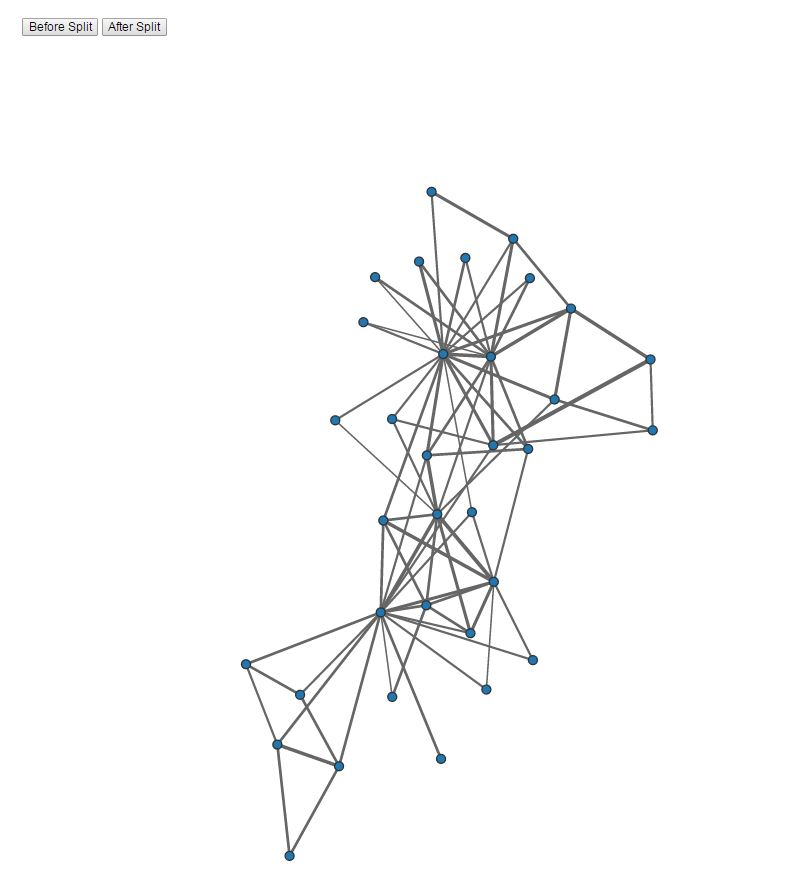
\includegraphics[scale=0.55, keepaspectratio=true]{figures/2.JPG}
\caption{Graph before split}
\label{fig:q3fig1}
\end{center}
\end{figure}
\newpage
\item   If we click on the button `After split' it generates a graph which differentiates 2 groups based on faction. This is illustrated in Figure \ref{fig:q3fig1}.
\begin{figure}[h!]
\begin{center}
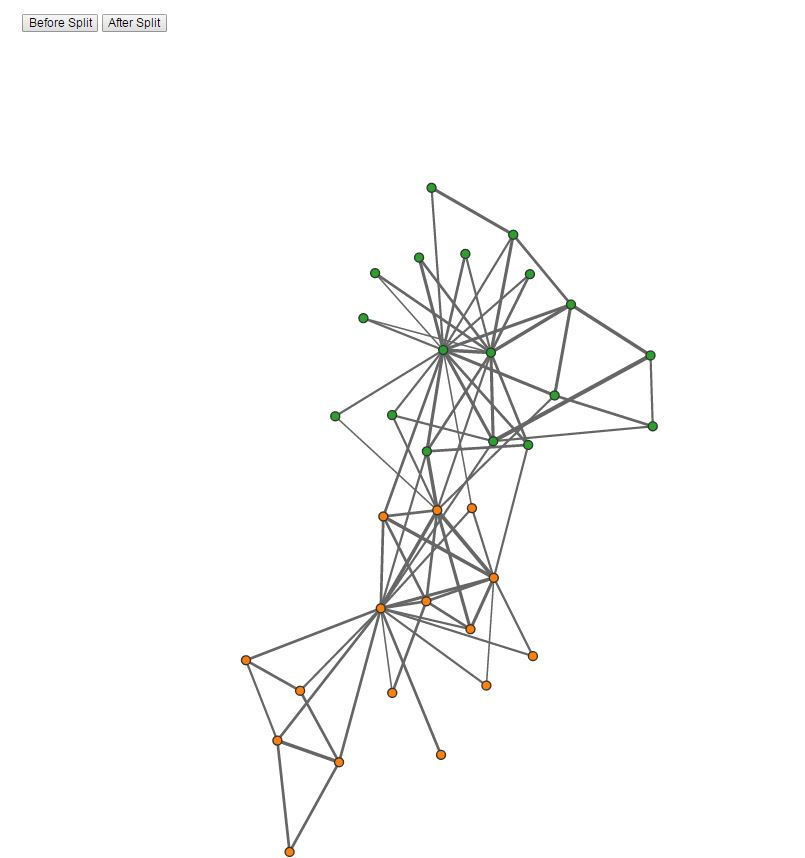
\includegraphics[scale=0.55, keepaspectratio=true]{figures/3.JPG}
\caption{Graph after split which distinguishes two groups based on Faction}
\label{fig:q1fig01}
\end{center}
\end{figure}
\end{itemize}

\newpage
\textbf{Code Listing}
\sloppy
\lstinputlisting[language=Python,caption=Python code for converting KarateClub XML graph to JSON data,frame=single,breaklines=true,label=lst:q3code1, tabsize=2, captionpos=b,numbers=left,showspaces=false,showstringspaces=false,basicstyle=\footnotesize]{src/xmlToJson.py}


